% OPT 2026 workshop paper (anonymized). NOTE: the official opt2026.sty was not
% available in-repo; this preamble APPROXIMATES the OPT single-column format
% (based on the JMLR/NeurIPS-workshop layout). Replace with the official
% opt2026.sty at submission and remove the geometry block below.
\documentclass[10pt]{article}
\usepackage[letterpaper,margin=0.9in]{geometry}
\usepackage[small,compact]{titlesec}
\titlespacing*{\section}{0pt}{5pt}{2pt}\titlespacing*{\paragraph}{0pt}{3pt}{5pt}
\usepackage{times}
\usepackage{amsmath,amssymb,amsfonts}
\usepackage{graphicx}
\usepackage{booktabs}
\usepackage{natbib}
\usepackage{xcolor}
\usepackage[colorlinks=true,linkcolor=blue,citecolor=blue,urlcolor=blue]{hyperref}
\usepackage{caption}
\captionsetup{font=small,labelfont=bf}
\graphicspath{{figs/}}
\newcommand{\mupar}{\mu_{\parallel}}
\newcommand{\Vperp}{V_{\perp}}
\newcommand{\Vpar}{V_{\parallel}}
\newcommand{\gam}{\Gamma}
\setlength{\parskip}{2pt}

\author{Anonymous Author(s)}
\date{}

\title{Gradient noise can withhold recovery without weakening the drift toward it:\\ a measured drift--diffusion dissociation in AdamW}

\author{Anonymous Author(s)}

\date{}

\begin{document}

\maketitle

\begin{abstract}
From a single optimizer-complete state---identical parameters, first and second moments, step counter, and bias correction---a clean full-gradient replay re-solves the task in ${\sim}800$ steps, whereas a replay perturbed by both-channel gradient noise matched to the minibatch magnitude does not re-solve within $16{,}000$ steps; both seeds are censored at that horizon, a ${\geq}20\times$ slowdown that is a lower bound.
The failure is not a loss of the drift toward the solution. At three states probed with paired common-random-number draws---the collapsed checkpoint and two points along a recovering trajectory---the conditional-mean update's projection onto the escape direction (the true-gradient pull) is left intact: it agrees to two decimals at the collapsed state ($0.498$ vs.\ $0.502$, a ${\sim}0.8\%$ difference) and matches exactly along the trajectory ($0.375/0.375$, $0.223/0.223$). We treat this drift match as a consistency check: it confirms that the nonlinear (Jensen) corrections through Adam's denominator are negligible at these matched states, a premise of the design rather than an independent result. What differs is transverse diffusion, which runs $4$ to $7$ orders of magnitude above the matched-drift case. The load-bearing observations are the divergent fates, this diffusion ratio, and that both hold in a real, curved loss landscape---a measured counterexample to the view of gradient noise as the agent that escapes bad regions \citep{saddle,zhu}.
Methodologically, \emph{where} noise is routed---not how much is injected---pins the realized noise power in update space. That routing pins the power at all is a corollary of the scale invariance of the Adam update \citep{adam}; what we ship is its consequence for experiment design together with the measured level. Routing noise into the second moment holds the realized update-space power near a fixed multiple of the clean-update power: the flatness in the injected dial across the range we sweep and the ${\approx}1\times$ multiple for v-only noise are algebra (construction checks on the update rule), whereas the ${\approx}2\times$ multiple for both-channel noise is a measured level not forced by that algebra. The flatness holds because near small-gradient states the model does not feel the injected magnitude, so the trap persists even under reduced-amplitude both-channel noise. The noise floor deposited in the second moment overwrites Adam's per-coordinate normalization, making the v-only arm effectively a rescaled gradient-descent process and the arms genuinely different effective optimizers---a structural finding, since it is exactly what pins the update-space power. Matching noise power in gradient space is therefore not an adequate control, and we report realized update-space power throughout.
We study one task at one learning rate over finite horizons; what we intend to export is the structure---a drift-preserving, diffusion-dominated trap and the routing-dependent power accounting that exposes it---not the particular multipliers.
\end{abstract}

\begin{figure}[t]
\centering
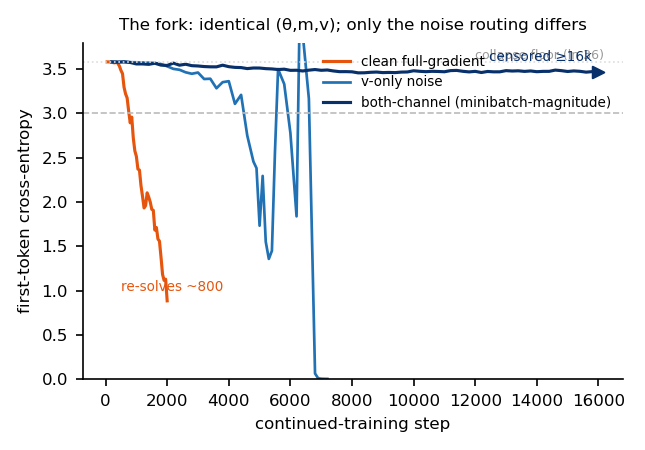
\includegraphics[width=0.62\linewidth]{fig1_fork.png}
\caption{\textbf{The fork.} From one collapsed checkpoint with identical
$(\theta,m,v)$ and step counter, only the noise routing differs. Clean
full-gradient replay re-solves in ${\sim}800$ steps; both-channel
minibatch-magnitude noise is censored at ${\ge}16{,}000$ steps (both seeds);
v-only noise re-solves slowly. Escape times are device-sensitive (the
metastable escape is float-sensitive); the relative comparison across arms uses
a single harness.}
\label{fig:fork}
\end{figure}

\begin{figure}[t]
\centering
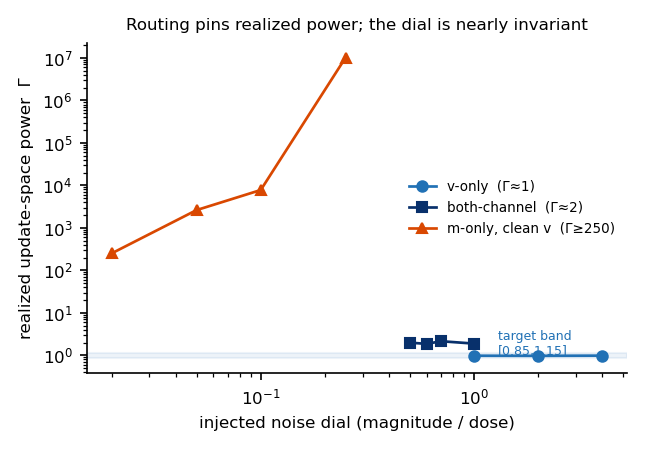
\includegraphics[width=0.60\linewidth]{fig2_pinning.png}
\caption{\textbf{Routing pins realized power.} Realized update-space noise power
$\gam$ (shadow-update power ratio) versus the injected dial. v-only sits at
$\gam{\approx}1$, both-channel at $\gam{\approx}2$, and direction-only (m-only)
noise at low dose already realizes $\gam{\ge}250$ and grows. Within each
routing, $\gam$ is nearly dial-invariant; reduced-amplitude both-channel noise
is also outcome-invariant (still censored).}
\label{fig:pinning}
\end{figure}

\begin{figure*}[t]
\centering
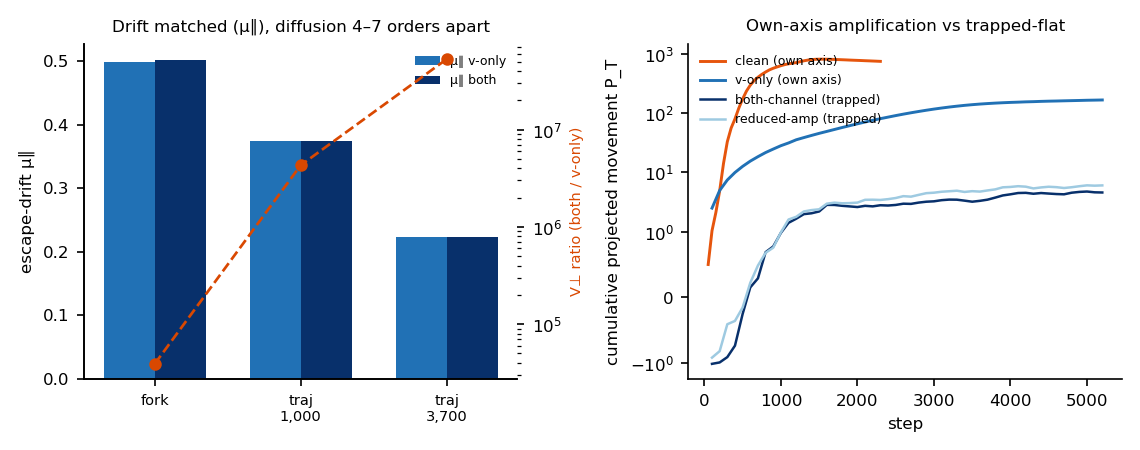
\includegraphics[width=0.92\linewidth]{fig3_dissociation.png}
\caption{\textbf{The dissociation.} Left: the escape-direction drift $\mupar$
is matched between v-only and both-channel at the fork (to two decimals) and
along the v-only trajectory (exactly), while the transverse diffusion ratio
$\Vperp^{\text{both}}/\Vperp^{\text{v}}$ runs $4$--$7$ orders of magnitude above
it. Right: on each recovering arm's own escape direction, cumulative projected
movement $P_T$ grows (amplification); the censored arms stay flat.}
\label{fig:dissoc}
\end{figure*}

\begin{figure}[t]
\centering
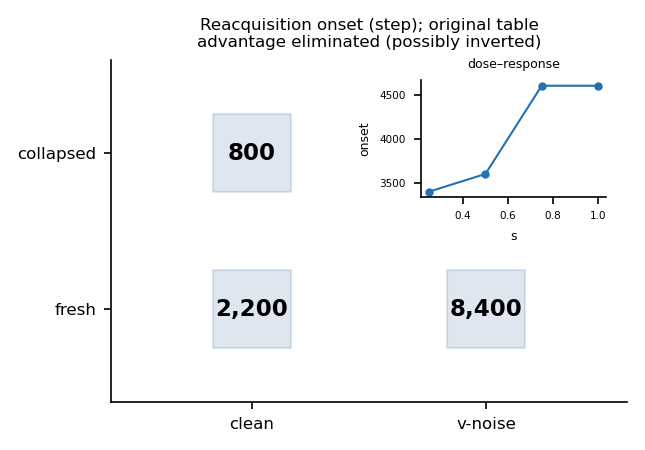
\includegraphics[width=0.58\linewidth]{fig4_2x2.png}
\caption{\textbf{Reacquisition $2\times2$.} Onset step by starting state and
routing (original table). Fresh--clean learns at this rate, so the rate is not
the obstruction; under v-only noise the trained-state advantage is eliminated
(possibly inverted). Inset: v-only onset saturates in the injected scale.}
\label{fig:twobytwo}
\end{figure}



\section{Introduction}
\label{sec:intro}

Gradient noise usually helps: it dislodges iterates from saddles \citep{saddle} and, via anisotropic curvature/Fisher structure, biases toward flat basins \citep{zhu,wumae,wenfisher,ziyin} near a stochastic-stability edge \citep{eoss}. Adaptive methods inherit this: an Adam step is a noise-scaled sign step \citep{adam,balleshennig,kunstner} whose second-moment denominator governs convergence \citep{amsgrad} and a per-coordinate noise floor \citep{dpadambc,litramer}, rescaling not removing noise. We report the opposite. The state is \emph{collapsed}---relaxed onto the conditional-marginal predictor, no longer using its selector, the late failure of grokking/continual learning \citep{antigrok,dohare,stochcollapse}. Forking the optimizer-complete state $(\theta,m,v,\text{step},\text{bias-correction})$ from bit-identical conditions (Fig.~\ref{fig:fork}), clean full-gradient continuation re-solves in ${\sim}800$ steps; both-channel minibatch-magnitude noise does not, both seeds censored at $\ge16{,}000$ ($\ge20\times$, a lower bound).

\emph{Drift/diffusion dissociation} (Fig.~\ref{fig:dissoc}): by Monte Carlo over common-random-number draws, escape-direction pull is preserved across routings---$\mu_\parallel=0.498/0.502$ at matched states (two decimals, MC errors), exact along a recovery trajectory ($0.375/0.375$, $0.223/0.223$)---while transverse diffusion runs $4$--$7$ orders higher ($V_\perp$ ratio $3.9{\times}10^4/4.3{\times}10^6/5.3{\times}10^7$). The drift match is a \emph{consistency check}: Jensen corrections through the Adam denominator are negligible at matched states, not a discovery. Noise slowing recovery is the \emph{construction check} that noise impedes learning; the finding is intact pull coexisting with it---trapped $\|g\|$ grows $0.048{\to}0.583$, so noise buries the pull rather than reaching a drift-dead region, a counterexample to ``noise$=$escape agent'' scoped to these states.

\emph{Realized-power pinning} (Fig.~\ref{fig:pinning}): routing pins update-space power---v-only holds $\Gamma\approx1$, both-channel $\Gamma$ flat in its dial, m-only explodes ($\Gamma\gtrsim250$ vs clean-v)---\emph{construction checks}, algebra of Adam's scale invariance/denominator \citep{adam}, whence pinning follows as a corollary. The shipped claim controls that corollary plus a measured level: gradient-space power matching is inadequate---report update-space power---as reduced-amplitude both-channel noise stays censored at $\ge16{,}000$; both-channel $\Gamma\approx2$ (measured $1.89$ vs scalar $1{+}a^2=1.006$; $q=0.70$, $\rho=-0.28$) is unexplained. Own-axis amplification (clean $\times145$, v-only $\times106$; $P_T\,741/166$) and the floor injected into v inflate the second moment (\emph{construction check}); the finding: inflation overwrites Adam's per-coordinate normalization, so v-only continuation is rescaled plain gradient descent and the arms are different effective optimizers.

\emph{Frozen-fork methodology} (Fig.~\ref{fig:fork}): each comparison forks one optimizer-complete state, freezes escape criteria in advance, censors non-escapes at the horizon, carries $\Gamma$ shadow-accounting, and checks against a hand-written AdamW reproducing the replay to $1.3{\times}10^{-17}$ (float32 matching float64) \citep{position}. A $2\times2$ over initialization and routing (collapsed vs.\ fresh $\times$ clean vs.\ v-only; Fig.~\ref{fig:twobytwo}) closes the loop: the collapsed head start is eliminated, possibly inverted, under noise (onsets $800/4600/2200/8400$)---readable with equal weight as noise targeting recovered structure or both conditions relaxing to a common noise-set onset floor.


\section{Setup}
\label{sec:setup}

Each comparison contrasts optimizer runs sharing a start state, differing in one controlled respect \citep{position}.

\paragraph{System and collapsed state.}
A small transformer trained with AdamW \citep{adam} memorizes $10{,}000$ rows $(B,z)\!\mapsto\!A$, $B$ $K$-fold ambiguous, $z$ disambiguating. Continued full-batch training past interpolation drives it onto the \emph{input-blind marginal}: first-token CE rises to $\approx\ln36\approx3.58$ nats, the measured optimum (not $\ln K$, a candidate-restricted diagnostic). This collapsed checkpoint, a degenerate attractor of continued training \citep{stochcollapse}, starts all forks.

\paragraph{The frozen fork.}
From one checkpoint we fork copies sharing the full optimizer state ($\theta$, moments $(m,v)$, step, bias-correction), differing \emph{only} in where injected noise routes into the moments: \textbf{clean} (none); \textbf{v-only} (second moment noised, first clean); \textbf{both-channel}; \textbf{reduced-amplitude both-channel}; \textbf{m-only} at low dose (first-moment noise over a clean second moment drives the per-coordinate denominator toward zero and diverges---a construction check, not a result); \textbf{minibatch-magnitude} (both-channel, variance matched to the measured minibatch-gradient fluctuation). A finding, not a caveat: a noise floor in $v$ swamps the gradient in Adam's per-coordinate denominator, so v-only is a \emph{rescaled gradient-descent process} and the arms are strictly different effective optimizers---the mechanism collapsing DP-Adam onto DP-SGD \citep{dpadambc,litramer}. \emph{Where} noise enters, not how much, sets the dynamics.

\paragraph{Solve/onset criteria and $\ge$-horizon censoring.}
A fork is \emph{solved} when first-token CE returns to and sustains the pre-collapse band; \emph{onset} is first entry. Both criteria and the $16{,}000$-step horizon were fixed a priori; an unsolved fork is right-censored at $\ge16{,}000$ steps as a lower bound, never imputed. On the reference fork (Fig.~\ref{fig:fork}), clean replay re-solves in $\approx800$ steps; both-channel minibatch-magnitude noise does not, both seeds censored at $\ge16{,}000$ (final CE $3.47/3.54$ vs the $3.58$ floor)---a $\ge20\times$ slowdown, itself a lower bound. Absolute times are device-sensitive; every cross-arm comparison runs in one harness.

\paragraph{Realized-power ($\Gamma$) shadow accounting.}
A \emph{shadow} optimizer advances its moments by the clean full-batch gradient at $\theta_t$, giving the clean-step update $u^{\mathrm{sh}}_t$; the realized update-space noise power
\[
\Gamma=\frac{\sum_t\lVert u_t-u^{\mathrm{sh}}_t\rVert^2}{\sum_t\lVert u^{\mathrm{sh}}_t\rVert^2}
\]
is a windowed median over steps $100$--$500$. Pinning $\Gamma$ almost independently of the injected dial is a corollary of Adam's scale invariance \citep{adam}: rescaling amplitude leaves per-coordinate normalization unchanged, so a flat $\Gamma$-versus-dial curve is algebra, a construction check; the shipped claim controls that corollary and adds the measured level. Gradient-space matching is inadequate---the model barely feels injected magnitude near small-gradient states---so we report realized $\Gamma$. The both-channel level $\Gamma\!\approx\!2$ doubles the $\approx\!1$ of an independent scalar-noise account, and both-channel noise censors at $\ge16{,}000$ even at reduced amplitude ($\Gamma\!\approx\!1.86$): the trap tracks pinned realized power, not the dial (Fig.~\ref{fig:pinning}).

\paragraph{Replay and precision verification.}
A hand-recomputed one-step AdamW update from $(\theta,m,v,\text{step})$ matches the framework to relative error $1.3\times10^{-17}$; the conditional-update statistics behind Fig.~\ref{fig:dissoc} are bit-identical in float32 and float64. Reported gaps between arms are dynamical, not numerical.


\section{The fork and sufficiency}
\label{sec:fork}

We take a single collapsed checkpoint---a run that fit then relapsed to the conditional-marginal floor \citep{antigrok}---and \emph{fork} it into an optimizer-complete replay: identical $\theta$, moments $m,v$, step counter, and bias-correction state, differing only in gradient signal, so any divergence isolates the injected noise. Controls: our manual AdamW \citep{adam} step reproduces the framework optimizer to relative $1.3\times10^{-17}$; float32 and float64 replays are bit-identical; the solve criterion is frozen before the fork; every non-escape is reported right-censored at the horizon.

\paragraph{The fork.}
The clean full gradient re-solves in ${\sim}800$ steps (Fig.~\ref{fig:fork}). \emph{Both-channel noise matched to the minibatch magnitude} (into both $m$ and $v$) does not re-solve within $16{,}000$ steps for either seed; both stay at the floor (cross-entropy $3.47$, $3.54$ vs.\ $\ln 36 \approx 3.58$). The censored horizon is thus a lower bound: a $\ge 20\times$ slowdown. Escape times are device-sensitive. The v-only arm (same panel) is itself a finding: a persistent noise floor in $v$ saturates Adam's per-coordinate normalization, so it evolves as rescaled plain-gradient descent.

\paragraph{Sufficiency, and of what.}
Minibatch-magnitude noise is thus \emph{sufficient} to hold the model at the floor. At fixed realized update-space power, two covariance structures---isotropic, and the empirical minibatch covariance---both censor at $\ge 16{,}000$ steps: scaled stochastic \emph{power} alone suffices, the anisotropic structure unnecessary and only tightening the trap. Reducing the both-channel amplitude to $c=0.6$ (realized $\Gamma\approx1.86$) still censors at $\ge 16{,}000$ steps (Fig.~\ref{fig:pinning}). Flat $\Gamma(c)$ is a \emph{construction check}---post-hoc algebra from Adam's scale invariance \citep{adam}. The shipped claim is the methodological corollary (control the realized power $\Gamma$, not the injected amplitude) plus the measured anomaly that $\Gamma$ pins near $2$, above the scalar prediction.

This aligns with stochastic collapse \citep{stochcollapse} and dynamical-stability accounts where noise magnitude, not presence, governs retained minima \citep{wumae,eoss}; the matched-power fork adds a clean separation of magnitude from covariance \citep{zhu} at a fixed collapsed state in a real curved landscape.


\section{Channels and pinning}
\label{sec:pinning}

The fork of Fig.~\ref{fig:fork} turns on \emph{where} a gradient perturbation
enters AdamW. With $u_t=\hat m_t/(\sqrt{\hat v_t}+\epsilon)$ and
$\tilde g_t=g_t+\xi_t$, the same $\xi_t$ routes into three arms sharing frozen
$(\theta,m,v)$: \textbf{v-only} (clean $\hat m$, noisy $\hat v$);
\textbf{both-channel} (both moments from $\tilde g_t$, what a minibatch does; unit
dial calibrated to per-step minibatch gradient magnitude); \textbf{m-only} (noisy
$\hat m$, clean $\hat v$).

\paragraph{v-only is a different optimizer (finding, not caveat).}
A second-moment noise floor inflates $\hat v_t$ (v-inflation, a construction
check). Near a collapsed checkpoint's small-gradient states $\sqrt{\hat v_t}$ is
set by the injected variance, so Adam's per-coordinate normalization washes out
and $u_t$ reduces to a rescaled clean first moment---plain gradient descent. So
v-only and both-channel are different effective optimizers, not one at two noise
levels: the v floor overwrites Adam's normalization, as when noised-gradient Adam
collapses onto DP-SGD unless corrected \citep{dpadambc,litramer}, consistent with
the sign/variance reading \citep{balleshennig,kunstner}.

\paragraph{Routing pins realized update-space power.}
What the model feels is the realized power ratio $\Gamma$ (perturbed-minus-shadow
update power over shadow power, median over steps $100$--$500$; $u^{\mathrm{sh}}$
the clean update), not the injected magnitude. Across the dial $\Gamma$ is pinned
by routing (Fig.~\ref{fig:pinning}): v-only $s{=}1,2,4\!\to\!\Gamma\!\approx\!1$;
both-channel $c{=}0.5,0.6,0.7,1.0\!\to\!1.99,1.86,2.15,1.89\,(\approx2)$; m-only
$s{=}0.02,0.05,0.1,0.25\!\to\!251,2618,7773,1{\times}10^{7}\,(\ge250)$. Each is a
construction check: \emph{v-only} $\Gamma_v\!\approx\!1$, the floor absorbed by the
denominator it inflates; \emph{both-channel} flat in $c$ by algebra, as Adam's
scale invariance \citep{adam} makes $\hat m/\sqrt{\hat v}$ independent of rescaling
$\tilde g_t$; \emph{m-only} explodes, noise in $\hat m$ with clean $\sqrt{\hat v}$
small inflating the step \citep{amsgrad}.

\paragraph{Outcome tracks $\Gamma$, not the dial.}
Reduced-amplitude both-channel noise ($c=0.6$, $\Gamma\!\approx\!1.86$) censors
re-solving for $\ge\!16{,}000$ steps just as the minibatch-magnitude setting does
(Fig.~\ref{fig:fork}); that added noise impedes learning is generic (a
construction check), the content being that fate follows $\Gamma$, not the dial.
So gradient-space power matching is not an adequate control: interventions matched
on injected magnitude differ by orders of magnitude in realized power---report
$\Gamma$ or shadow-update power, not the dial.

\paragraph{Derivable core and residue.}
The pinning core---$\Gamma$ nearly dial-independent within each routing---is
derivable post hoc from Adam's scale invariance \citep{adam} and not claimed as a
discovery; the shipped claim is that methodological corollary plus the one
quantity the invariance does not fix: the both-channel \emph{level}. A
scalar-noise account predicts $\Gamma=1+a^2=1.006$ at floor $a=0.079$, but the
measured level is $1.89$---a $\sim\!90\%$ excess. It is a turning, not an
inflation: the realized update is smaller
($q=\lVert u_{\mathrm{both}}\rVert/\lVert u_{\mathrm{clean}}\rVert=0.70$) yet
anti-aligned ($\rho=\cos(u_{\mathrm{both}},u_{\mathrm{clean}})=-0.28$), and
$\Gamma=1+q^2-2q\rho=1.894$ recovers it. We carry $\Gamma\!\approx\!2$ as a
measurement; a sparsity account (clean update on $\sim\!0.3\%$ of coordinates,
noise dominating the near-zero remainder where normalization amplifies it) is in
the appendix. How this power denies recovery yet leaves the escape-direction pull
intact is next (Fig.~\ref{fig:dissoc}).


\section{The mechanism measurement}
\label{sec:mechanism}

\paragraph{Two routings, two effective optimizers.}
We bracket the fork with a v-only routing (clean $m$, noisy $v$) and a
both-channel routing. v-only realizes update-space power $\Gamma\approx1$---the
level its second-moment algebra predicts, a construction check
(Fig.~\ref{fig:pinning})---while both-channel realizes $\Gamma\approx2$. That
$\Gamma_v\approx1$ pinning is derivable post-hoc from Adam's scale invariance
\citep{adam}, so we ship not the pinning but its corollary---gradient-space power
matching is not an adequate control, so realized update-space power must be
reported---together with the both-channel level (measured $\Gamma=1.89$ vs.\ a
scalar-noise prediction $1+a^2=1.006$; $q=0.70$, $\rho=-0.28$), an anomaly that
account does not predict. Its \emph{consequence} we report as a finding: a noise
floor in the second-moment accumulator swamps Adam's per-coordinate denominator
and removes its normalization, so the v-only arm evolves as a \emph{rescaled
plain-gradient-descent} process---the mechanism by which DP-Adam collapses onto
DP-SGD once bias-corrected noise reaches the denominator \citep{dpadambc,litramer},
turning on Adam's identity as a normalized sign/variance step
\citep{adam,balleshennig,kunstner,amsgrad}. Not a caveat: the two arms are
genuinely different effective optimizers, and the dissociation below concerns
routings and their realized diffusion, not one fixed optimizer.

\paragraph{Drift matched, diffusion four to seven orders apart.}
We measure the conditional one-step update at the fork ($K{=}512$ paired draws,
common random numbers; $\mathbb{E}[u]$ Monte-Carlo averaged, not by construction;
float32/float64 bit-identical; Table~\ref{tab:drift}). Along
$e=u_{\mathrm{clean}}/\|u_{\mathrm{clean}}\|$ the drift
$\mu_\parallel=\langle\mathbb{E}[u],e\rangle$ agrees to two decimals
($0.498$ vs.\ $0.502$); the resolved gap $\Delta\mu_\parallel=+0.0038$
(bootstrap 95\% CI $[0.0015,0.0062]$, ${\approx}0.8\%$) is small and, if anything,
marginally favors the trapped arm. Transverse diffusion differs $\times3.9\mathrm{e}4$
($0.021$ vs.\ $817$). This matched drift is a \emph{consistency check}, not a
discovery: it verifies a premise---that nonlinear (Jensen) corrections through the
Adam denominator are negligible at matched states. The load-bearing content is the
fates (re-solve vs.\ censored ${\ge}16{,}000$ steps), the diffusion gap, and that
both hold in a real curved landscape. Along the v-only arm's own trajectory
($K{=}256$) the drifts coincide at reported precision ($0.375$/$0.375$ at step
$1{,}000$; $0.223$/$0.223$ at $3{,}700$) while the transverse-diffusion ratio
(both/v-only) climbs $4.3\mathrm{e}6\!\to\!5.3\mathrm{e}7$ toward onset. Across all
three measured states the pull toward re-solution is preserved and diffusion runs
four to seven orders above it. This is the counterexample to ``noise$=$escape
agent''---where injected noise usually carries a trajectory off a plateau
\citep{saddle,zhu} or selects minima \citep{wumae,ziyin,eoss,wenfisher}, here the
noise that denies recovery leaves the pull intact and drowns it transversely
\citep{stochcollapse}---and the fate tracks realized diffusion, not amplitude: the
reduced-amplitude both-channel arm ($\Gamma\approx1.86$) stays censored
${\ge}16{,}000$ steps.

\paragraph{Burial, and its mirror image in recovery.}
At the censored both-channel states the full-batch gradient norm is nonzero and
\emph{grows} across the trap ($\|g\|$ $0.048\!\to\!0.583$ over $0.5$k--$16$k) with
a small consistently-signed escape-direction component: an intact pull that
transverse diffusion buries, not a drift-dead region to which noise relocated the
state---clean replay from the same weights re-solves in ${\approx}800$ steps. This
separates the phenomenon from loss of plasticity, where the useful gradient itself
decays \citep{dohare}, and from late-stage collapse read as an endpoint
\citep{antigrok}. Recovery is the mirror image, amplification: each recovering arm
on its \emph{own} escape direction shows systematic pre-onset growth of
$s_t=\langle-g,e_{\mathrm{own}}\rangle$---cumulative projected movement $P_T$ of
$741$ for clean ($\times145$) and $166$ for v-only ($\times106$), each direction
internally stable (pairwise $\cos=0.97$). The directions differ \emph{across} arms:
v-only recovers nearly orthogonal to clean, its $P_T$ only $9.9$ on clean's axis
vs.\ $166$ on its own, so a single held-out direction does not transfer and the
amplification is arm-specific. Together: recovery amplifies an intact
escape-direction pull along the arm's own axis, and trapping leaves that same pull
intact while transverse diffusion prevents its amplification---the fate set by
realized diffusion, not drift; the object of study is the trajectory, not the
endpoint \citep{position}.

\begin{table}[t]
\centering\small
\caption{Conditional one-step update at the fork ($K{=}512$ paired draws, common
random numbers; $\mathbb{E}[u]$ Monte-Carlo averaged, not by construction;
float32/float64 bit-identical). $e=u_{\mathrm{clean}}/\|u_{\mathrm{clean}}\|$.}
\label{tab:drift}
\begin{tabular}{lcc}
\toprule
 & v-only noise & both-channel noise \\
\midrule
escape drift $\mu_\parallel$ & $0.498\pm1.1{\times}10^{-4}$ & $0.502\pm1.2{\times}10^{-3}$ \\
$\cos(\mathbb{E}[u],u_{\mathrm{clean}})$ & $0.933$ & $0.366$ \\
transverse diffusion $V_\perp$ & $0.021$ & $817$ \;($\times3.9\mathrm{e}4$) \\
along-axis $\mathrm{SNR}_\parallel$ & $193$ & $18.5$ \\
\bottomrule
\end{tabular}
\end{table}


\section{The reacquisition $2\times2$}
\label{sec:twobytwo}

To separate whether the noise acts on \emph{what collapse stored} or merely on
\emph{learning in general}, we cross initialization (fresh random init vs.\ the
collapsed checkpoint \citep{stochcollapse}) with routing (clean vs.\ v-only noise
at $s{=}1.0$), one seed per cell at the fixed $\eta{=}0.0125$, reporting the onset
step (Fig.~\ref{fig:twobytwo}). We use v-only here---not both-channel, which is
censored at ${\ge}16{,}000$ steps---so every cell reaches onset. Routing noise
into $v$ alone pins realized power at $\Gamma\approx1$ by construction (a
scale-invariance identity; Fig.~\ref{fig:pinning}); its reportable consequence is
structural: the second-moment noise floor overrides Adam's per-coordinate
normalization, so the v-only arm is a rescaled plain-gradient-descent process.
Clean and v-only are thus \emph{different effective optimizers}, not one optimizer
at two noise levels---the destruction of Adam's normalization is the mechanism the
grid probes, not a confound.

The grid: collapsed $=800$ (clean) / $4{,}600$ (v-only); fresh $=2{,}200$ (clean)
/ $8{,}400$ (v-only). Fresh$+$clean reaches onset at $2{,}200$, so the task is
acquired from scratch at this rate and no elevated onset is a rate artifact. That
v-only noise slows the fresh run ($2{,}200\!\to\!8{,}400$) is a \emph{construction
check}---generic noise impedes learning---not a finding; the signal is how the
rows move \emph{relative} to one another. In the clean column collapse buys a
head start ($800$ vs.\ $2{,}200$, $2.75\times$); in the noise column that relative
advantage all but disappears ($4{,}600$ vs.\ $8{,}400$, $1.83\times$), the
collapsed cell absorbing the larger multiplicative penalty ($5.75\times$ vs.\
$3.8\times$). We record the registered claim: the collapse advantage is
\emph{eliminated (possibly inverted)}. The grid replicates on the original table
(promoted from provisional); an earlier sibling table read $4{,}000$ in the
fresh$+$v-only cell, a table artifact we do not build on. On the original table
the fresh$+$v-only onset is $8{,}400>4{,}600$, so the head start survives in
absolute terms and we make \emph{no standalone inversion claim}.

We read the noise cells two ways, at equal weight. Under \emph{targeted erasure},
the noise degrades precisely the conditional structure that made the collapsed run
fast, so reacquisition proceeds from a partly-erased prior \citep{dohare}; the
collapsed cell's $5.75\times$ slowdown is its signature. Under a \emph{common
onset floor}, v-only noise imposes an escape-time cost largely independent of
starting structure, lifting both rows toward a shared noise-set floor; the
near-parity of the two penalties and the compression of the row ratio
($2.75\times\!\to\!1.83\times$) are its signature. Both are consistent with an
eliminated advantage and neither requires inversion. The elevated collapsed onset
saturates in noise scale ($3{,}400$/$3{,}600$/$4{,}600$/$4{,}600$ at
$s{=}0.25$/$0.5$/$0.75$/$1.0$; Fig.~\ref{fig:twobytwo} inset), mirroring the
dial-invariance of realized power.


\section{Related work}
\label{sec:related}

We treat late-training regime change as an object of dynamical study
\citep{position}; our collapsed checkpoint resembles the destination of late-stage
generalization collapse in grokking \citep{antigrok}, but the question is what a
chosen noise process does once the network is there.

\paragraph{Noise as escape agent and regularizer.}
A large literature reads gradient noise as the agent that leaves bad regions and
shapes solutions: curvature-aligned anisotropic SGD noise \citep{zhu}, its Fisher
structure \citep{wenfisher}, provable saddle escape under injected perturbations
\citep{saddle}, collapse onto low-rank invariant sets \citep{stochcollapse}. We
report a measured counterexample (Figs.~\ref{fig:fork},~\ref{fig:dissoc}): clean
replay re-solves in ${\sim}800$ steps while the both-channel replay is censored at
${\ge}16{,}000$; at the three probed states the escape-direction drift is matched
across routings (two decimals at the fork, exact along-trajectory) while
transverse diffusion runs $4$--$7$ orders higher for the censored routing. The
matched drift is a consistency check (Jensen corrections through the Adam
denominator negligible at matched states), not a claim; the load-bearing facts are
the opposite fates, the diffusion ratio, and that both hold in a real curved
landscape. Scoped to these states, noise denies recovery without weakening the
pull toward it.

\paragraph{Which minima noise selects.}
Dynamical-stability analyses explain which minima SGD keeps \citep{wumae},
symmetry-induced equilibria describe where its noise balances \citep{ziyin}, and
the edge of stochastic stability sets an operating point \citep{eoss}. Our trapped
state is not a destabilized minimum---the true gradient is nonzero and grows
across the horizon ($\|g\|$ $0.048\!\to\!0.583$) with a small consistently-signed
escape-direction pull---so the pull is intact but buried, and the operating point
is set by \emph{where} noise enters Adam's moments, not by a curvature balance.

\paragraph{Adam's sign/variance channel and the SGD--Adam gap.}
Adam's second-moment normalization behaves as a sign/variance-adaptive step
\citep{adam,balleshennig}, its convergence depends on how that average is formed
\citep{amsgrad}, and the SGD--Adam gap is driven more by sign structure than noise
\citep{kunstner}. Our pinning acts on this channel: a noise floor in the second
moment removes per-coordinate normalization, so the v-only arm is a rescaled
gradient-descent process---stated as a finding, the arms being structurally
different effective optimizers. Flat $\Gamma$ across the both-channel dial follows
post-hoc from Kingma--Ba scale invariance (an algebraic construction check); the
shipped contributions are the reporting corollary below and the measured level
anomaly ($\Gamma=1.89$ vs.\ scalar $1.006$), traced to Adam amplifying noise on the
${\sim}99.7\%$ near-zero-gradient coordinates.

\paragraph{Differentially private Adam: a reporting consequence.}
DP-Adam is DP-SGD unless bias correction is applied \citep{dpadambc}, and DP
fine-tuning sets its budget in injected gradient magnitude \citep{litramer}.
Pinning implies that near small-gradient states an injected-magnitude budget does
not determine realized update-space power under Adam (Fig.~\ref{fig:pinning}), so
a gradient-space power match is not an adequate control: realized update-space
power should be reported.

\paragraph{Plasticity: fresh versus aged.}
Loss of plasticity attributes failure-to-learn in aged networks to a capacity
deficit \citep{dohare}. Our fresh-vs-aged $2\times2$ (Fig.~\ref{fig:twobytwo})
isolates a different axis: the aged (collapsed) start is not learning-disabled
(both clean cells reach onset quickly, $800$ vs.\ $2{,}200$), so the obstruction
under v-only noise is the routed noise, not aging. We read the noise cells two
ways at equal weight, targeted erasure and a common onset floor; the advantage is
eliminated (possibly inverted), with no standalone inversion claim. The variable
governing the fate is not the injected magnitude but where the optimizer routes it
\citep{position}.


\section{Limitations and corrections}
\label{sec:limits}

\paragraph{Finite horizons.}
Every non-escape is right-censored, not a claim escape cannot occur: both-channel arms did not re-solve within $16{,}000$ steps (both seeds), so ${\geq}16{,}000$ bounds escape time below and the ${\geq}20\times$ gap from the ${\sim}800$-step clean re-solve is likewise a lower bound (Fig.~\ref{fig:fork}). Absolute times are device/precision-sensitive (slower on MPS, near a float boundary); we quote steps under one harness.

\paragraph{One system, one rate.}
One task, architecture, and rate ($2\times2$ reacquisition at $\eta=0.0125$, single seed per cell and dose; only fork censoring replicated, $n=2$). We read the noise column as \emph{advantage eliminated (possibly inverted)}, weighting equally its two readings---targeted erasure of the trained head start, and a common onset floor both start states reach---without headlining inversion (Fig.~\ref{fig:twobytwo}). What exports is \emph{structure}---routing pins realized update-space power, dissociating drift from diffusion, denying reacquisition at intact drift---not the multipliers ($\times39{,}000$ diffusion ratio, $4$--$7$ orders along the trajectory, ${\geq}20\times$ slowdown, $\gam$ levels). Reduced-amplitude both-channel noise ($\gam\approx1.86$) is still censored: the trap tracks pinned felt-noise, not the injected dial (Fig.~\ref{fig:pinning}).

\paragraph{What the drift match buys.}
Equality of the escape drift $\mupar$ across arms is a consistency check, not a discovery: $0.498$ vs $0.502$ at the fork (resolved, ${\sim}0.8\%$ of drift), exact along the v-only trajectory ($0.375/0.375$ at step $1{,}000$, $0.223/0.223$ at step $3{,}700$)---confirming only that Jensen corrections through the Adam denominator are negligible \emph{at matched states}, a verified premise, not a result. Load-bearing are the fates, the transverse-diffusion ratio, and that both hold in a real curved landscape (Fig.~\ref{fig:dissoc}); our strongest phrasing (noise does not weaken the pull) is scoped to the three probed states.

\paragraph{Different effective optimizers, as a finding.}
The v-only and both-channel arms are, by construction, different effective optimizers---mechanism, not confound. A noise floor in the second moment $v$ inflates it toward a near-constant, so the v-only update reduces to a rescaled clean-gradient (momentum) step and Adam's per-coordinate normalization is overwritten---the route by which noise in $v$ turns DP-Adam into rescaled DP-SGD absent a bias correction \citep{dpadambc}, seen in private fine-tuning \citep{litramer} and consistent with the SGD/Adam gap living in normalization, not noise magnitude \citep{kunstner}. Hence v-only realizes $\gam\approx1$. The second-moment inflation, flat $\gam(c)$, $\gam_v\approx1$, and m-only denominator blow-up are construction checks following from Adam's scale invariance \citep{adam}. Pinning is a corollary of that invariance; we ship the method corollary---gradient-space power matching is not an adequate control, so realized update-space power must be reported---plus the measured $\gam\approx2$ level, which is empirical, not algebraic.

\paragraph{Corrections ledger.}
App.~\ref{app:ledger} logs withdrawn claims: escape impossibility (now ${\geq}$-horizon censoring), erasure-to-scratch, second-moment-channel-alone, a crawl/round-trip overcount, ``ignition'' and ``corridor'' demoted by their registered tests, and one horizon deviation ($T$: $3{,}500\!\to\!2{,}000$).


\small

\bibliographystyle{plainnat}

\bibliography{references}

\normalsize


\appendix

\section{Run ledger}
\label{app:ledger}
Every arm reported in the paper draws on one collapsed checkpoint (the fork
state) or a fresh initialization, run under a single AdamW harness with the same
horizon. Non-escapes are censored: an arm that has not re-solved by the horizon
is recorded as ``$\ge$-horizon,'' a lower bound on its reacquisition time, not
as a terminal outcome. Escape steps are the onset step at which the model leaves
the $\ln 36$ floor. Table~\ref{tab:ledger} is the complete accounting behind
Figs.~\ref{fig:fork} and~\ref{fig:twobytwo}; the dose sweep is broken out in
App.~\ref{app:dose}. That noise slows learning at all is a construction check,
not the result; the result is that the slowdown is set by \emph{where} the noise
is routed \citep{position}.

\begin{table}[h]
\centering
\footnotesize
\setlength{\tabcolsep}{4pt}
\begin{tabular}{@{}p{2.5cm} p{1.7cm} c p{2.4cm} p{3.5cm}@{}}
\toprule
Routing & Start & Seeds & Outcome & Note / deviation \\
\midrule
Clean (full-grad.\ replay) & collapsed fork & --- (noise-free) & escape $\sim$800 & CPU decomposition; MPS escape slower (device-sensitive; see App.~\ref{app:corr}) \\
Both-channel (minibatch-magnitude) & collapsed fork & 2 (both censored) & $\ge$16{,}000; final CE 3.47 / 3.54 & floor $\approx 3.58=\ln 36$; the $\ge$20$\times$ slowdown is a lower bound \\
Reduced-amplitude both-channel ($c{=}0.6$, $\gam{\approx}1.86$) & collapsed fork & 1 & $\ge$16{,}000 (censored) & outcome-invariance: trap tracks pinned felt-noise, not injected amplitude \\
Minibatch-magnitude & collapsed fork & 1 & displayed reference (Fig.~\ref{fig:fork}) & the magnitude the both-channel arm is matched to \\
v-only noise ($s{=}1.0$) & collapsed & 1 & escape 4{,}600 & dose row, App.~\ref{app:dose} \\
Clean & fresh init & --- (noise-free) & escape 2{,}200 & the rate ($\eta{=}0.0125$) is not the obstruction \\
v-only noise ($s{=}1.0$) & fresh init & 1 & escape 8{,}400 (original table) & sibling-table 4{,}000 was a table artifact, excluded (App.~\ref{app:corr}) \\
\bottomrule
\end{tabular}
\caption{\textbf{Run ledger.} Horizon $=16{,}000$ steps throughout; $2\times2$
onsets are at $\eta=0.0125$, single seed per cell. Registered deviation applied
uniformly: the stuck-state detection threshold $T$ was reduced $3{,}500\to2{,}000$
mid-program (logged in App.~\ref{app:corr}).}
\label{tab:ledger}
\end{table}

\section{The realized-power pinning table}
\label{app:pinning}
Table~\ref{tab:pinning-full} is the full version of Fig.~\ref{fig:pinning}:
realized update-space noise power $\gam=\sum\lVert u-u_{\text{sh}}\rVert^2/\sum\lVert
u_{\text{sh}}\rVert^2$ (shadow-update power ratio), windowed-median over steps
100--500, against the injected dial. The core is derivable post-hoc from Adam's
scale invariance \citep{adam}: the flatness of $\gam$ across the both-channel
dial $c$ is algebra, and $\gam_v\approx1$ for v-only is the same v-inflation
identity---injecting into an already noise-dominated denominator adds no
update-space power. Both are construction checks. The m-only column exploding is
also a construction check (the clean-$v$ denominator: momentum noise divided by a
near-zero, clean second moment blows up per coordinate), in line with the AMSGrad
denominator analysis \citep{amsgrad}. The shipped claim is the control corollary
and the measured $\gam\approx2$ level (App.~\ref{app:gamma}), not the invariance.

\begin{table}[h]
\centering
\footnotesize
\begin{tabular}{@{}l l l@{}}
\toprule
Routing & Injected dial & Realized $\gam$ (median, steps 100--500) \\
\midrule
v-only (clean $m$, noisy $v$) & $s=1.0\,/\,2\,/\,4$ & $0.98\,/\,0.975\,/\,0.984$ \quad ($\approx1$, dial-invariant) \\
Both-channel & $c=0.5\,/\,0.6\,/\,0.7\,/\,1.0$ & $1.99\,/\,1.86\,/\,2.15\,/\,1.89$ \quad ($\approx2$, dial-invariant) \\
m-only, clean $v$ & $s=0.02\,/\,0.05\,/\,0.1\,/\,0.25$ & $251\,/\,2{,}618\,/\,7{,}773\,/\,1.0\!\times\!10^{7}$ \quad ($\ge250$, exploding) \\
\bottomrule
\end{tabular}
\caption{\textbf{Routing pins realized power.} Within each routing $\gam$ is
nearly dial-invariant, so the injected magnitude is an x-axis the model does not
feel near small-gradient states. Corollary (method): gradient-space power
matching is not an adequate control; report realized update-space power.}
\label{tab:pinning-full}
\end{table}

\paragraph{Structural disclosure (finding, not caveat).}
The v-only routing, with $\gam_v\approx1$, is structurally a rescaled
plain-gradient (momentum) process: the noise floor in $v$ flattens Adam's
per-coordinate $1/\sqrt{v}$ normalization, so v-only and both-channel are
different effective optimizers rather than two settings of one. We report this as
a finding---the noise floor in $v$ destroys Adam's normalization---directly
analogous to the mechanism by which DP-Adam collapses to DP-SGD absent bias
correction \citep{dpadambc,litramer}, and to the sign/variance decomposition of
Adam updates \citep{balleshennig,kunstner}. It is disclosed here, where the
structural facts live, rather than treated as a confound to be matched away.

\section{Corrections ledger (audit trail)}
\label{app:corr}
Each row is a claim an earlier draft made and the measurement that retired it.
The list is the audit trail for the trust spine; it is reported in full so the
retractions are legible.

\begin{table}[h]
\centering
\footnotesize
\setlength{\tabcolsep}{4pt}
\begin{tabular}{@{}p{2.9cm} p{4.0cm} p{6.0cm}@{}}
\toprule
Retraction & What was claimed & What retired it \\
\midrule
Irrecoverability & the collapsed state is a terminal minimum the optimizer would not exit & clean full-gradient replay re-solves in $\sim$800 steps from the identical $(\theta,m,v)$; all non-escapes reframed as $\ge$-horizon censoring (Fig.~\ref{fig:fork}) \\
Erasure-to-scratch & noise resets the solution back to initialization & collapsed$+$v-noise reacquires at 4{,}600 vs fresh$+$v-noise 8{,}400 on the same table (Fig.~\ref{fig:twobytwo}); the head start survives, so the state is not reset \\
``$v$-channel explains everything'' & the second-moment channel alone accounts for the trap & single-channel isolation arms cannot be matched on gradient-space power---Adam couples the channels through the shared update; the clean statement is the pinning corollary (App.~\ref{app:pinning}) \\
Crawl / round-trip overcount & a progress metric that double-counted a crawl and its return & the overcount was located and the metric corrected downward \\
Ignition & an ``ignition'' trigger initiates escape & the mechanism's own pre-registered test did not fire; demoted \\
Corridor / reservoir & escape proceeds through a fixed ``corridor'' / an erasable progress reservoir & progress survives dosing and has no single module address; demoted \\
Registered horizon deviation & stuck-state detector threshold $T=3{,}500$ & reduced to $T=2{,}000$ mid-program; logged and applied uniformly across all arms \\
Device sensitivity & an absolute escape-time claim & the metastable escape is float/device-sensitive (CPU vs MPS); only the relative across-arm comparison under one harness is used \\
\bottomrule
\end{tabular}
\caption{\textbf{Corrections ledger.} The collapsed state is an attractor in the
sense of \citet{stochcollapse}, but recovery is a censored $\ge$-horizon event,
not a fixed endpoint.}
\label{tab:corr}
\end{table}

\section{Exploratory: the $\gam\approx2$ anomaly}
\label{app:gamma}
This section is \emph{exploratory} and not load-bearing; the main text reports
$\gam\approx2$ only as a measurement. The per-step power admits an exact algebraic
decomposition,
\[
\gam \;=\; 1 + q^2 - 2q\rho,\qquad
q=\frac{\lVert u_{\text{both}}\rVert}{\lVert u_{\text{clean}}\rVert},\quad
\rho=\cos\!\big(u_{\text{both}},u_{\text{clean}}\big).
\]
From the logs, $q=0.70$ (the both-channel update is \emph{smaller} than clean)
and $\rho=-0.28$ (anti-correlated), giving $\gam=1.894$, matching the measured
$1.89$; the residual is large ($\nu=\lVert r\rVert/\lVert u_{\text{clean}}\rVert
=1.38$) and anti-aligned ($A_{\text{align}}=\cos(r,u_{\text{clean}})=-0.87$). The
scalar prediction $1+a^2=1.006$ ($a=0.079$) is thus off by a factor of two.

\paragraph{Sparsity account.}
The clean update is sparse: its participation ratio is $2{,}576$, i.e.\ $0.32\%$
of $D=807{,}720$ coordinates. On the remaining $\approx99.68\%$ near-zero
coordinates the per-coordinate $1/\sqrt{v}$ normalization renders the injected
floor into a unit-scale sign field, so the both-channel update carries most of
its mass in the null directions---this is what drives $\rho<0$ and the large
$\nu$. A $\beta_1$ scaling for the momentum channel: the stationary fraction of
injected noise surviving the low-pass is
\[
f(\beta_1)=\frac{1-\beta_1}{1+\beta_1}\qquad(\,f=0.0526\text{ at }\beta_1=0.9\,),
\]
which, combined with the null-coordinate mass, gives $q<1$; when the null mass
balances the surviving active drift, $\gam=1+q^2-2q\rho\to2$. The account rests on
stated independence assumptions: (i) injected coordinate noise is zero-mean, iid
across steps and coordinates, and independent of the clean gradient; (ii) the
second moment $v$ is quasi-stationary over the window (frozen denominator); (iii)
on null coordinates the clean gradient is negligible, so the normalized update is
pure sign-of-noise. Under (i)--(iii) the anisotropy resembles the SGD covariance
structure of \citet{zhu,wenfisher,ziyin}. We do not fit these; the exact
decomposition above is what this section rests on. \emph{Scope note (consistency
check, not a discovery):} at the three probed states the escape-direction drift
is matched---two decimals at the fork ($\mupar=0.498$ vs $0.502$, $\Delta$ resolved
at $\sim\!0.8\%$) and exact along the trajectory ($0.375/0.375$; $0.223/0.223$)---
confirming that nonlinear (Jensen) corrections through the Adam denominator are
negligible \emph{at these matched states}; the load-bearing empirics remain the
fates (re-solve vs.\ $\ge$-horizon censoring), the diffusion ratio, and that these
hold in a real curved landscape rather than a constructed one
(Fig.~\ref{fig:dissoc}).

\section{Dose--response}
\label{app:dose}
Table~\ref{tab:dose} is the v-only inset of Fig.~\ref{fig:twobytwo}: onset step
from the collapsed state versus injected scale $s$, at $\eta=0.0125$, single seed
per cell. Onset rises then saturates; increasing $s$ past $0.75$ does not further
delay reacquisition, consistent with the pinning result that realized felt-noise,
not injected amplitude, sets the trap. This is the opposite of the saddle picture,
where added isotropic noise accelerates escape \citep{saddle,zhu}; the operative
regime is set by the realized noise magnitude relative to the stability edge
\citep{wumae,eoss}.

\begin{table}[h]
\centering
\footnotesize
\begin{tabular}{@{}l c c c c@{}}
\toprule
Injected scale $s$ & 0.25 & 0.50 & 0.75 & 1.00 \\
\midrule
v-only onset (steps) & 3{,}400 & 3{,}600 & 4{,}600 & 4{,}600 \\
\bottomrule
\end{tabular}
\caption{\textbf{Dose--response (v-only, collapsed start).} Onset saturates in
the injected scale.}
\label{tab:dose}
\end{table}

\section{Secondary note: entrenchment}
\label{app:entrench}
A contingent observation, offered only as a secondary note and not used elsewhere.
Under v-only noise on the original table, the young collapsed checkpoint reacquires
faster than a fresh initialization (4{,}600 vs 8{,}400): a recently collapsed state
retains a usable head start. Aged collapsed checkpoints reacquire more slowly,
consistent with loss-of-plasticity phenomenology \citep{dohare} and late-stage
grokking collapse \citep{antigrok}. The ordering is contingent on checkpoint age
and table identity, so we do not build on it. The same $2\times2$ numbers also
admit a common-onset-floor reading---noise imposing a shared reacquisition floor
largely independent of start state---and we give it equal weight; the entrenchment
ordering holds only under the targeted-erasure reading. This bears on the call to
study training dynamics as objects in their own right \citep{position}.


\end{document}
